\documentclass[submitting]{nst}

\usepackage{subfigure,dcolumn}
\usepackage[T2A,T1]{fontenc}
\usepackage[russian,english]{babel}

% The following package will be used to typeset the LaTeX codes and is not a necessity to this template
\usepackage{listings}
\lstloadlanguages{[LaTeX]TeX}
\lstset{language=[LaTeX]TeX,keywordstyle=\color{red},showspaces=true,breaklines=true,breakatwhitespace=true,basicstyle=\small\tt,commentstyle=\color{white},frame=single,framerule=0pt,backgroundcolor=\color{yellow}}


\begin{document}


\title{Titles should be no more than three typeset lines (generally 135 characters including spaces) and should be comprehensible to a broad scientific audience (replace with your real title)}\thanks{Supported by the National Natural Science Foundation of China (No.xxxxxxxx) and the Major State Basic Research Development Program of China~(No. yyyyyyyy)}

\author{Zhi-Chu Chen}
\affiliation{Shanghai Institute of Applied Physics, Chinese Academy of Sciences, Shanghai 201800, China}
\affiliation{Shanghai Synchrotron Radiation Facility, Chinese Academy of Sciences, Shanghai 201204, China}
\author{Yi Zhang}
\affiliation{Shanghai Institute of Applied Physics, Chinese Academy of Sciences, Shanghai 201800, China}
\affiliation{Shanghai Synchrotron Radiation Facility, Chinese Academy of Sciences, Shanghai 201204, China}
\author{Doe John}
\email[Corresponding author, ]{The name, complete address, telephone number, and e-mail address of the author to whom correspondence and proofs should be sent. E-mail addresses will appear in print and online.}
\affiliation{Author affiliation. Include department, institution, and complete address, with the ZIP/postal code, for each author. Use superscripts to match authors with institutions.}



\begin{abstract}
 NST publishes theoretical and experimental studies in all aspects of nuclear science and technology. This guide is intended to be a handbook as well as a template for the authors who are ready to submit their manuscripts to NST. A complete manuscript submission contains the following items: title, author affiliation, corresponding author, abstract, keywords, introduction, experimental section, results and discussion, conclusion, acknowledgments and references. The Introduction should provide a statement outlining the motivation for the research and should accurately place the investigations in context with previous or current work in the field.  The experimental section should provide a clear, unambiguous description of materials, methods, and equipment in sufficient detail to permit repetition of the work elsewhere. Repetitive descriptions of a general procedure should be avoided. Results and discussion should present the results, and their interpretation, in context with existing knowledge in a clear and concise manner. The conclusion section should be provided in instances where the key elements of the results and discussion may require amplification or clarification. This section should not simply restate the Abstract. References must be in NST style. Only published or in-press papers and books may be cited in the reference list. Unpublished abstracts of papers presented at meetings or references to ``data not shown'' are not permitted. Each literature reference should be assigned one number and placed in the text as a Arabic numeral. Unnecessarily long reference lists should be avoided.
\end{abstract}


\keywords{Keywords are listed below the abstract of the manuscript. At least three keywords are required at submission.}

\maketitle


\section{Introduction}

NST, founded in 1990, is a unique journal published in English in the field of nuclear research in China. This periodical is devoted to the publication of fundamental research papers. Coverage in NST spans all aspects of nuclear science and technology including theories, experiments and applications. A special interest lies in the subjects of synchrotron radiation applications, beam line technology, low energy accelerator, ray technology and applications,nuclear chemistry, radiochemistry and radiopharmaceuticals and nuclear medicine, nuclear electronics and instrumentation, nuclear physics and interdisciplinary research, nuclear energy science and engineering as well.

Published bimonthly since 2004, NST has been playing a role of increasing importance to promote academic exchanges between nuclear scientists of China and other countries, and it has contributed quite a bit to the development of nuclear science and techniques and their applications in China. NST is sponsored by Shanghai Institute of Applied Physics, Chinese Academy of Sciences and has been indexed by SCI-E, CA in US, SA in UK and \foreignlanguage{russian}{РЖ} in Russia.


\section{Figures}\label{sec:artwork}

Provide figure images in EPS, JPEG, PNG or GIF format; Color images must be in RGB (red, green, blue) mode. Images must be final size, preferably one column width (\SI{8.5}{\centi\metre}). Figures wider than one column should be between 10.5 and \SI{16.0}{\centi\metre} wide. Numbers, letters, and symbols should be 7 points after reduction and must be consistent.
 
Submitted raster images must meet the minimum resolution requirements. Raster images can be classified as monochrome (line-art), halftone, or combination halftone.
\begin{description}

\item[Monochrome (1-bit) images (line drawing)] Common examples are graphs and charts made of solid black and white, with no gray values. The preferred resolution for this type of image is between 1000 and 1200 dpi at publication size.
\item[Combination Halftones] Common examples are color or grayscale figures containing halftone and line art elements. The preferred resolution for this type of image is between 600 and 900 dpi at publication size.
\item[Halftones] Common examples are color or grayscale figures containing pictures only, with no text or thin lines. The suggested minimum resolution for this type of image is 300 dpi at publication size.
\end{description}

The graphics could be wrapped in the \texttt{figure} float environment. The word ``float'' means that the location of the block will be determined by the program by using an aesthetical algorithm. 

For example, if a figure is wrapped in \verb|\begin{figure}[!htb]...\end{figure}|, \LaTeX\ will try to put it in the current place. If \LaTeX\ thinks it is not an appropriate place, it will try to put it at the top of the current page. If that fails as well, it will try to put it at the bottom of the page. What happens is not really important to the authors, but it is always a good idea to put a block of contents in a float environment such as figures and tables.

If an external figure file is wanted to be included in the article, the \verb|\includegraphics{filename}| macro will be used. The title of the figure can be specified by using the \verb|\caption{Caption contents...}| and a cross reference anchor \verb|\label{key}| is preferred to be following the \verb|\caption| macro. The cross reference is yet another powerful tool used by \LaTeX. Once a \verb|\label| is set, the ordinal and the page number can be referred by using \verb|\ref{key}| and \verb|\pageref{key}| anywhere within the article and they will be synchronizing without further interfering.

A full example is shown in listing~\ref{lst:fig} and produces the Fig.~\ref{fig:one-column-figure}. The \verb|draft| key used here is only because this template comes without \verb|file.png| and this key would draw a frame box to illustrate how the picture would be inserted and it's always not used in practical writings. the \verb|width| key will scale the width of the picture to 80\%\ of the text width, keeping the ratio between the width and the height. A really wide picture could be inserted by using the \verb|figure*| environment as shown in Fig.~\ref{fig:two-columns-figure}. 

\begin{lstlisting}[caption={Source code of Figure~\ref{fig:one-column-figure}},label=lst:fig]
\begin{figure}[!htb]
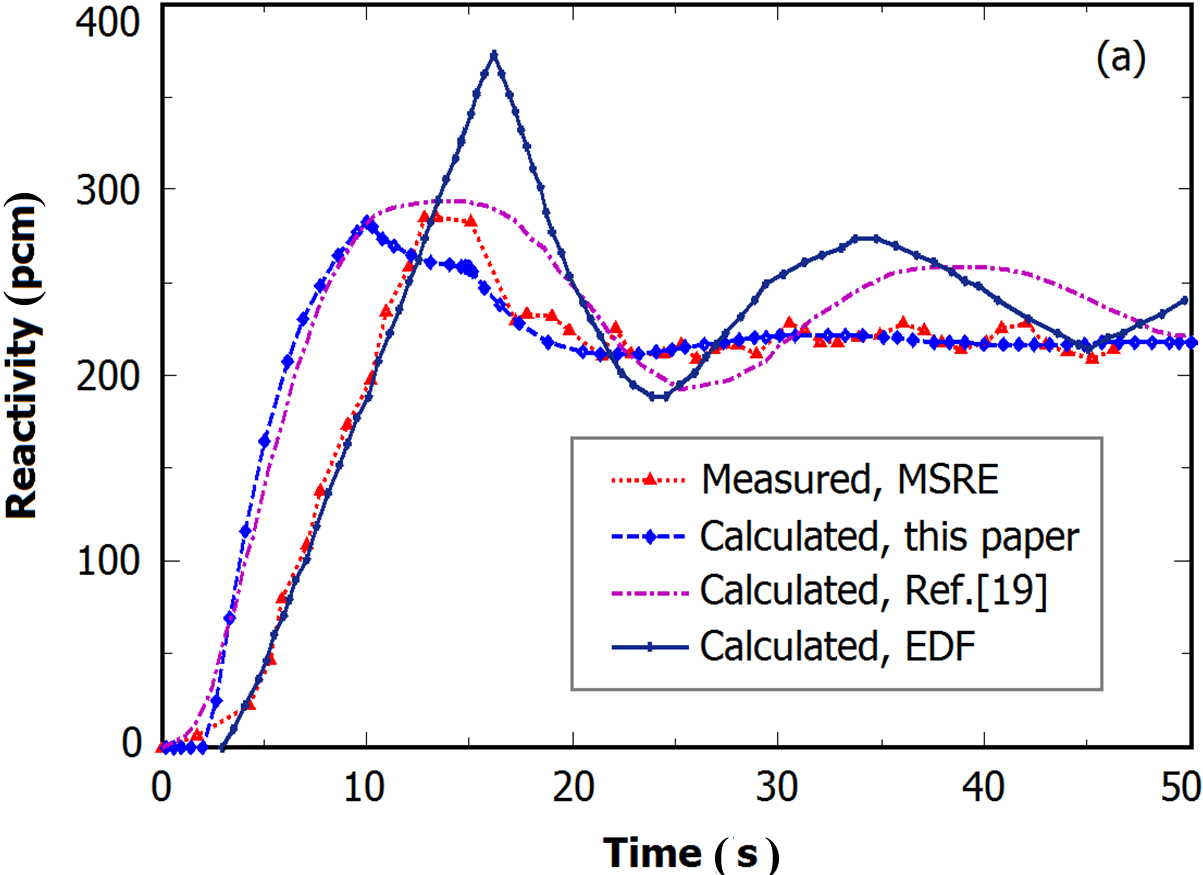
\includegraphics
  [draft,width=0.8\hsize]
  {file.png}
\caption{A well-prepared line drawing reduced to the journal column width.}
\label{fig:one-column-figure}
\end{figure}
\end{lstlisting}

\begin{figure}[!htb]
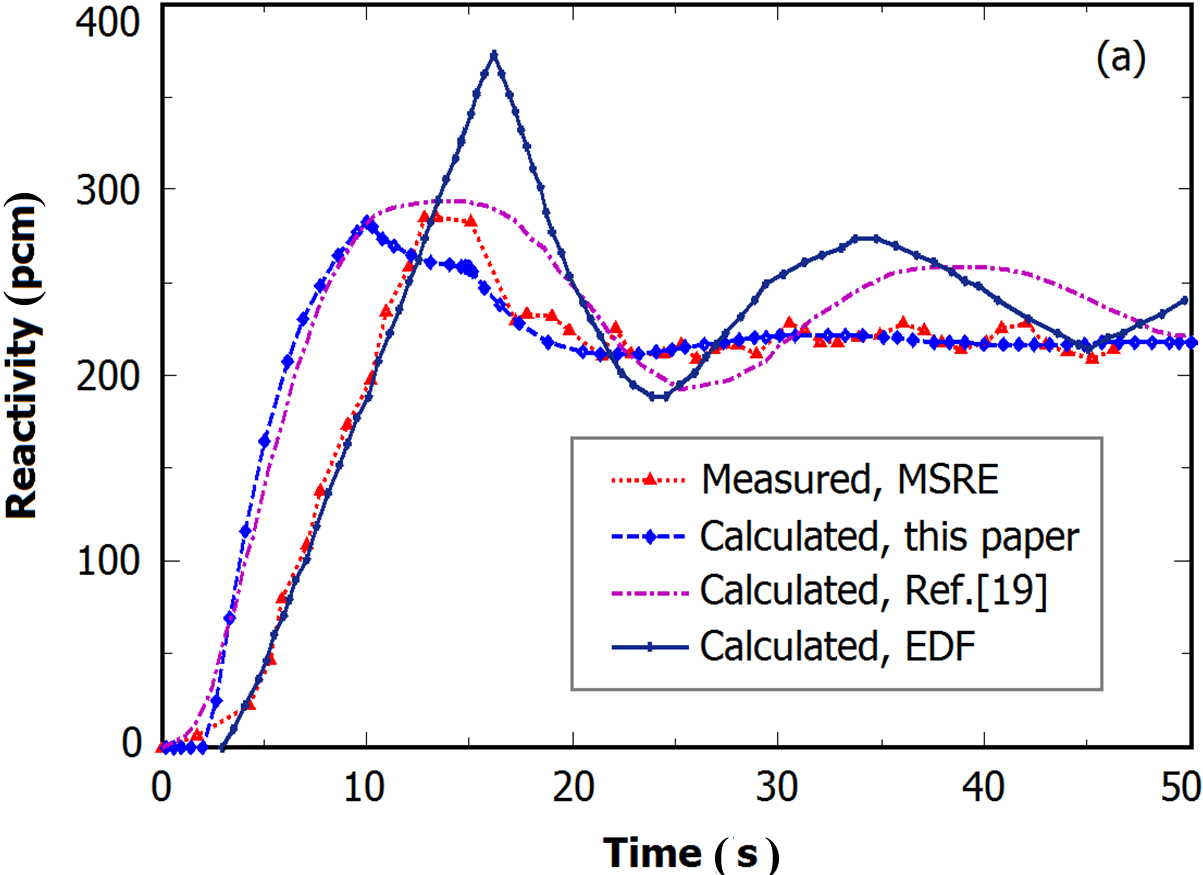
\includegraphics
  [width=0.45\hsize]
  {file.png}
\caption{A well-prepared line drawing reduced to the journal column width.}
\label{fig:one-column-figure}
\end{figure}

\begin{figure*}[!htb]
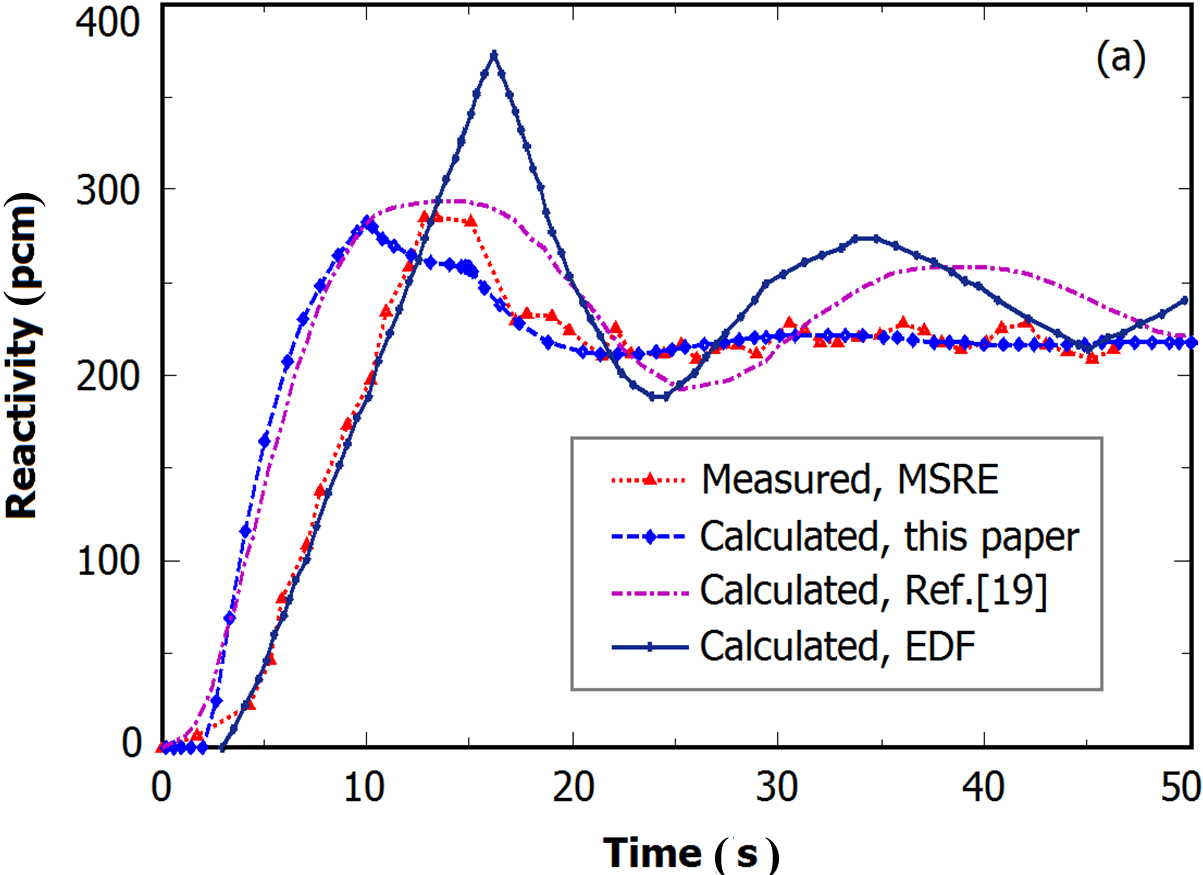
\includegraphics
  [width=0.9\hsize]
  {file.png}
\caption{The actual size of a well-prepared line drawing.}
\label{fig:two-columns-figure}
\end{figure*}

\begin{lstlisting}[caption={Source code of Figure~\ref{fig:two-columns-figure}},label=lst:fig2]
\begin{figure*}[!htb]
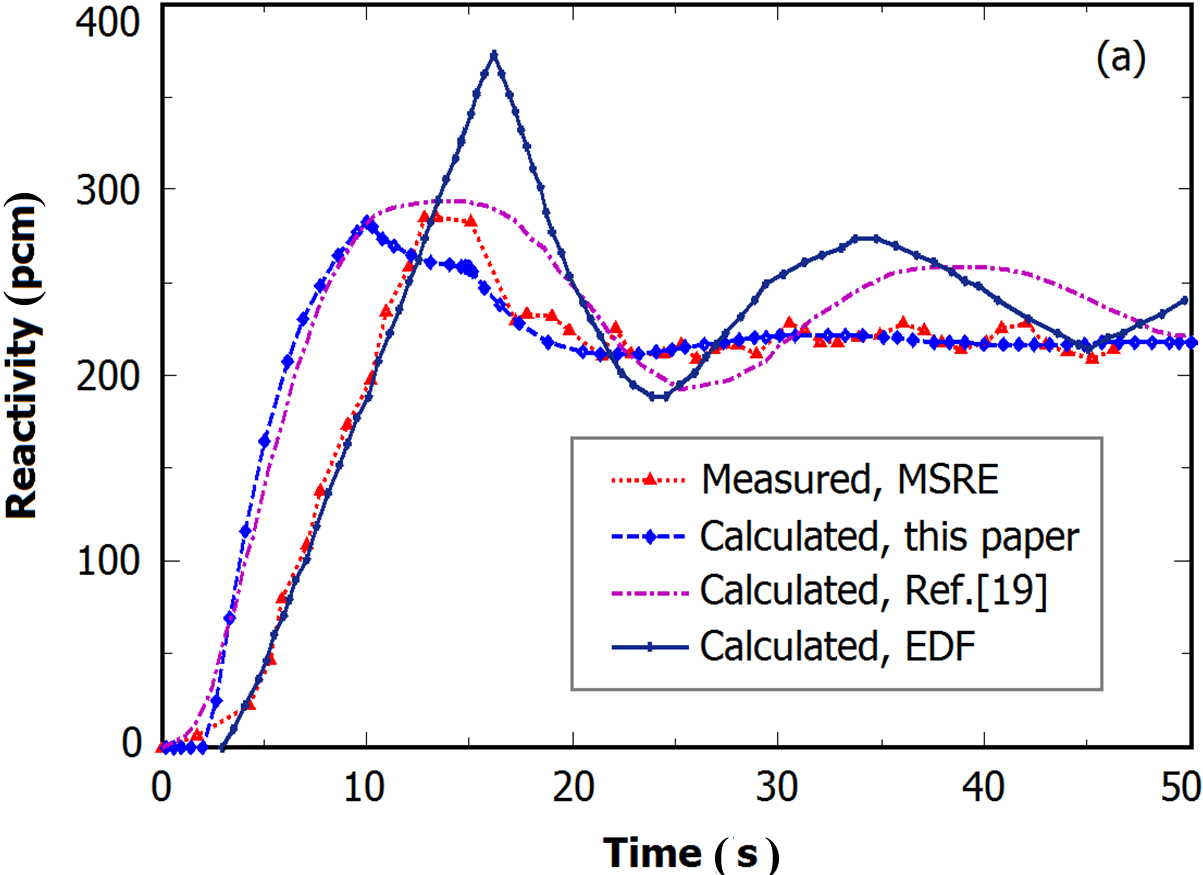
\includegraphics
  [width=0.9\hsize]
  {file.png}
\caption{The actual size of a well-prepared line drawing.}
\label{fig:two-columns-figure}
\end{figure*}
\end{lstlisting}


\section{Tables}

Tables should be numbered consecutively with Arabic numerals and placed in appropriate locations within the text. Each table should include a descriptive heading that, together with the individual column headings, makes the table self-explanatory. Footnotes in tables should be given letter designations and be cited in the table by superscript letters. The sequence of letters should proceed by line rather than by column.

To provide professional, publication quality tables, vertical rules are prohibited as illustrated in table~\ref{tab:animal-price}. The source code is shown in listing~\ref{lst:tab}. The \texttt{Table} environment provides a float environment~(please refer to Sec.~\ref{sec:artwork}, and like the \verb|figure| environment, the \verb|table| environment also has the star-version environment \verb|table*|) for the tabular and the \texttt{\char`\\label} macro provide the cross reference anchor for further usage. The \texttt{tabular} environment draws the table here and the parameter \texttt{llr} means that this table has three columns: the first two columns will be left aligned and the last column will be right aligned. The \texttt{\char`\\toprule}, \texttt{\char`\\cmidrule}, \texttt{\char`\\midrule} and \texttt{\char`\\bottomrule} draw the top, middle and bottom rules respectively. The \texttt{\&} symbol is the delimiter of the table, separating the columns and the \texttt{\char`\\\char`\\} means the end of a row.

\begin{table}[!htb]
\caption{The caption of the table goes here.}
\label{tab:animal-price}
\begin{tabular*}{8cm} {@{\extracolsep{\fill} } llr}
\toprule
\multicolumn{2}{c}{Item} \\
\cmidrule(r){1-2}
Animal & Description & Price (\$) \\
\midrule
Gnat  & per gram & 13.65 \\
      & each     &  0.01 \\
Gnu   & stuffed  & 92.50 \\
Emu   & stuffed  & 33.33 \\
Armadillo & frozen & 8.99 \\
\bottomrule
\end{tabular*}
\end{table}

\begin{lstlisting}[caption={Source code of Table~\ref{tab:animal-price}},label=lst:tab]
\begin{table}[!htb]
\caption{The caption of the table goes here.}
\label{tab:animal-price}
\begin{tabular*}{8cm} {@{\extracolsep{\fill} } llr}
\toprule
\multicolumn{2}{c}{Item} \\
\cmidrule(r){1-2}
Animal & Description & Price (\$) \\
\midrule
Gnat  & per gram & 13.65 \\
      & each     &  0.01 \\
Gnu   & stuffed  & 92.50 \\
Emu   & stuffed  & 33.33 \\
Armadillo & frozen & 8.99 \\
\bottomrule
\end{tabular*}
\end{table}
\end{lstlisting}


\section{Units}

The SI system should be used for all scientific and laboratory data. 
To typeset the SI units, two commands\footnote{These commands are provided by the \texttt{siunitx} package which has been taken care of by the NST class automatically.} can be handy: \texttt{\char`\\SI\{}\textit{num}\texttt{\}\{}\textit{unit}\texttt{\}} and \texttt{\char`\\si\{}\textit{unit}\texttt{\}}. For example, \verb|\SI{3e8}{\metre\per\second}| gives \fbox{\SI{3e8}{\metre\per\second}} and \verb|\si{\micro\ampere}| gives \fbox{\si{\micro\ampere}}. Abbreviations are also supported so that \verb|\si{m/s}| and \verb|\si{kg.m/s^2}| will be converted to the corresponding symbols correctly. For more information, please read \href{http://ftp.ctex.org/mirrors/CTAN/macros/latex/contrib/siunitx/siunitx.pdf}{the manual of the \texttt{siunitx} package}.


\section{Math}
\subsection{In-line math}

The in-line math symbols or equations can be typeset by putting them in the \verb|$...$| blocks. For example, \texttt{\$\char`\\mathcal\{F\} = \char`\\frac\{1\}\{\char`\\sqrt\{2\char`\\pi\}\} \char`\\int\_\{-\char`\\infty\}\char`\^\{\char`\\infty\} \char`\\mathrm\{d\}t e\char`\^\{i\char`\\omega t\}\$} will produce $\mathcal{F} = \frac{1}{\sqrt{2\pi}} \int_{-\infty}^{\infty} \mathrm{d}t e^{i\omega t}$. The display math formula can be obtained by using the \verb|equation| environment as shown in listing~\ref{lst:eq} and Eq.~\eqref{eq:structure-constants-of-Lie-algebra-1}.

\begin{lstlisting}[caption={Source code of Equation~\eqref{eq:structure-constants-of-Lie-algebra-1}},label=lst:eq]
\begin{equation}\label{eq1}
C_{ab}^b = -C_{ba}^b = +2, \quad
C_{ac}^c = -C_{ca}^c = -2, \quad
C_{bc}^a = -C_{cb}^a = +1 .
\end{equation}
\end{lstlisting}

\begin{equation}\label{eq:structure-constants-of-Lie-algebra-1}
C_{ab}^b = -C_{ba}^b = +2, \quad C_{ac}^c = -C_{ca}^c = -2, \quad C_{bc}^a = -C_{cb}^a = +1 .
\end{equation}


\subsection{Wide Contents}

If in such circumstances that the contents are too wide for the column, the authors are encouraged to use the \verb|widetext| environment to put these in. We can see that both listing~\ref{lst:eq} and Eq.~\eqref{eq:structure-constants-of-Lie-algebra-1} are a little wider than the width of the text so that a more esthetically acceptable way would be using the code in listing~\ref{lst:eq:wide}. 

\begin{widetext}
\begin{lstlisting}[caption={Source code of Equation~\eqref{eq:structure-constants-of-Lie-algebra-1:widetext}},label=lst:eq:wide]
\begin{widetext}
\begin{equation}\label{eq:structure-constants-of-Lie-algebra-1}
C_{ab}^b = -C_{ba}^b = +2, \quad
C_{ac}^c = -C_{ca}^c = -2, \quad
C_{bc}^a = -C_{cb}^a = +1 .
\end{equation}
\end{widetext}
\end{lstlisting}
\end{widetext}

And get the output as in Eq.~\eqref{eq:structure-constants-of-Lie-algebra-1:widetext}. 

\begin{widetext}
\begin{equation}\label{eq:structure-constants-of-Lie-algebra-1:widetext}
C_{ab}^b = -C_{ba}^b = +2, \quad C_{ac}^c = -C_{ca}^c = -2, \quad C_{bc}^a = -C_{cb}^a = +1 .
\end{equation}
\end{widetext}


\section{Bibliography}

The \verb|thebibliography| environment provides a cross reference way to cite the bibliographies. Its only parameter is used to determine the label width and an article referring 10--99 references will always use \verb|99| as the parameter. The entries will be labeled by the \verb|\bibitem| and referred with \verb|\cite|. This template fakes 20 references labeled from \verb|bib:1| to \verb|bib:20|\footnote{Actually, this is not a good way to label your references without any actual meanings. The author of the guide uses \texttt{bib:\textit{author}:\textit{year}:\textit{journal}:\textit{volume}:\textit{number}} to label his references and an adequate editor~(he uses TeXstudio and emacs)} and the command \verb|\cite{bib:1}| will cite the first entry\cite{bib:1} and \texttt{\char`\\cite\{bib:2, bib:3, bib:4, bib:5, bib:6, bib:7, bib:8, bib:9, bib:10, bib:20, bib:19, bib:18, bib:17, bib:15, bib:14, bib:13, bib:12, bib:11\}} will sort and compress the entries\cite{bib:2, bib:3, bib:4, bib:5}


\begin{thebibliography}{99}
\bibitem{bib:1} C. Simenel, P. Chomaz, G. de France, Quantum calculation of dipole excitation in fusion reaction. Phys. Rev. Lett. {\bf 86}, 2971--2974 (2001). \href{http://dx.doi.org/10.1103/PhysRevLett.86.2971}{doi: 10.1103/PhysRevLett.86.2971}
\bibitem{bib:2} C. Tao, Y. G. Ma, G. Q. Zhang, \emph{et al}., Pygmy and giant dipole resonances by Coulomb excitation using a quantum molecular dynamics model. Phys. Rev. C, {\bf 87}: 014621 (2013). \href{http://dx.doi.org/10.1103/PhysRevC.87.014621}{DOI: 10.1103/PhysRevC.87.014621} 
\bibitem{bib:3} D.M. Abrams, in {\it Conductive Polymers}, ed. by R.S. Seymour, A. Smith (Springer, Berlin Heidelberg New York, 1973), p. 307 
\bibitem{bib:4} H. Ibach, H. Lüth, {\it Solid-State Physics}, 2nd edn. (Springer, New York, 1996), pp. 45–56 
\bibitem{bib:5} D. Zowghi et al., in {\it PRICAI '96: Topics in Artificial Intelligence}, ed. by N. Foo, R. Goebel. 4th Pacific Rim Conference on Artificial Intelligence, Cairns, August 1996. Lecture Notes in Computer Science. Lecture notes in artificial intelligence, vol. 1114 (Springer, Heidelberg, 1996), p. 157 
\end{thebibliography}



\end{document}